\documentclass[usenames,dvipsnames]{beamer}

\mode<presentation> {

% The Beamer class comes with a number of default slide themes
% which change the colors and layouts of slides. Below this is a list
% of all the themes, uncomment each in turn to see what they look like.

%\usetheme{default}
% \usetheme{AnnArbor}
%\usetheme{Antibes}
%\usetheme{Bergen}
% \usetheme{Berkeley}
% \usetheme{Berlin}
%\usetheme{Boadilla}
%\usetheme{CambridgeUS}
% \usetheme{Copenhagen}
\usetheme{Darmstadt}
% \usetheme{Dresden}
% \usetheme{Frankfurt}
% \usetheme{Goettingen}
%\usetheme{Hannover}
%\usetheme{Ilmenau}
%\usetheme{JuanLesPins}
%\usetheme{Luebeck}
% \usetheme{Madrid}
% \usetheme{Malmoe}
%\usetheme{Marburg}
% \usetheme{Montpellier}
% \usetheme{PaloAlto}
% \usetheme{Pittsburgh}
%\usetheme{Rochester}
% \usetheme{Singapore}
%\usetheme{Szeged}
%\usetheme{Warsaw}

% As well as themes, the Beamer class has a number of color themes
% for any slide theme. Uncomment each of these in turn to see how it
% changes the colors of your current slide theme.

% \usecolortheme{albatross}
%\usecolortheme{beaver}
%\usecolortheme{beetle}
%\usecolortheme{crane}
%\usecolortheme{dolphin}
%\usecolortheme{dove}
%\usecolortheme{fly}
\usecolortheme{lily}
%\usecolortheme{orchid}
%\usecolortheme{rose}
%\usecolortheme{seagull}
%\usecolortheme{seahorse}
%\usecolortheme{whale}
%\usecolortheme{wolverine}

%\setbeamertemplate{footline} % To remove the footer line in all slides uncomment this line
%\setbeamertemplate{footline}[page number] % To replace the footer line in all slides with a simple slide count uncomment this line

\setbeamertemplate{navigation symbols}{} % To remove the navigation symbols from the bottom of all slides uncomment this line
}

% % -------------------------------------------
% % Songkai added, feel free to delete --------
% \AtBeginSection[]{
%   \begin{frame}
%   \vfill
%   \centering
%   \begin{beamercolorbox}[sep=8pt,center,shadow=false,rounded=true]{title}
%     \usebeamerfont{title}\insertsectionhead\par%
%   \end{beamercolorbox}
%   \vfill
%   \end{frame}
% }
% % Songkai added, feel free to delete --------
% % -------------------------------------------




\usepackage{graphicx} % Allows including images
\usepackage{booktabs} % Allows the use of \toprule, \midrule and \bottomrule in tables
\usepackage{natbib}
\usepackage{amsmath, amssymb, graphicx, url}
\usepackage[ruled]{algorithm2e}
\usepackage{commath}
\usefonttheme[onlymath]{serif}

\usepackage{amsmath}
\usepackage{amssymb}
\usepackage{centernot}
\usepackage{comment}
%\usepackage[a4paper, margin=0.8in]{geometry}
\usepackage{parskip}
\usepackage{graphicx}

\usepackage{natbib}

\usepackage{tikz}
\usepackage{tikzlings}

\usepackage{tabularx}
\usepackage{array}
\usepackage{multirow}
\usepackage{makecell}
\usepackage{mathtools}
\usepackage{bm,upgreek}
\usepackage{subcaption}
\usepackage{textpos}
% \usepackage{eso-pic}

% \usepackage{multimedia}
\usepackage{media9}

\def\E{\mathbf{E}}
\def\PP{\mathbf{P}}
\def\Reals{\mathbb{R}}
\def\Naturals{\mathbb{N}}
\def\argmin{\operatornamewithlimits{arg\,min}}
\def\deq{:=}
\def\wh#1{\widehat{#1}}
\def\bd#1{\mathbf{#1}}
\def\bx{\bd{x}}
\def\by{\bd{y}}
\def\bZ{\bd{Z}}
\def\bB{\bd{B}}
\def\bV{\bd{V}}
\def\tO{{\tilde{\cO}}}
\def\tOm{\tilde{\Omega}}
\def\barw{\overline{w}}
\def\d{{\mathrm d}}
\def\ave#1{\langle #1 \rangle}
\def\Ave#1{\left\langle #1 \right\rangle}
\def\eps{\varepsilon}
\def\tr{\mathrm{Tr}}


\def\HS{\mathbb{H}}
\def\reals{\mathbb{R}}
\def\ths{\theta^*}
\def\thh{\hat{\theta}}
\def\lbr{\left[}
\def\rbr{\right]}
\def\lc{\left(}
\def\rc{\right)}


    \def\ddefloop#1{\ifx\ddefloop#1\else\ddef{#1}\expandafter\ddefloop\fi}
    % \cA, \cB, ...
    \def\ddef#1{\expandafter\def\csname c#1\endcsname{\ensuremath{\mathcal{#1}}}}
    \ddefloop ABCDEFGHIJKLMNOPQRSTUVWXYZ\ddefloop
    \def\argmin{\operatornamewithlimits{arg\,min}}
    \def\E{\mathbf{E}}
    \def\bx{\bd{x}}
	\def\by{\bd{y}}
    \def\bZ{\bd{Z}}

\newcommand{\propnumber}{} % initialize
\newtheorem*{prop}{Proposition \propnumber}
\newenvironment{propc}[1]
  {\renewcommand{\propnumber}{#1}%
   \begin{shaded}\begin{prop}}
  {\end{prop}\end{shaded}}

\newcommand{\crlrnumber}{} % initialize
%\newtheorem*{corollary}{Corollary \crlrnumber}
\newenvironment{corollaryc}[1]
  {\renewcommand{\crlrnumber}{#1}%
   \begin{shaded}\begin{corollary}}
  {\end{corollary}\end{shaded}}

\theoremstyle{definition}
% \newtheorem{definition}




% \setbeamertemplate{headline}{% 
%     \leavevmode%
%     \hbox{%
%         \begin{beamercolorbox}[wd=.4\paperwidth,ht=2.25ex,dp=1ex,right]{section in head/foot}%
%             \usebeamerfont{section in head/foot}\insertshorttitle\hspace*{2ex}
%         \end{beamercolorbox}%
%         \begin{beamercolorbox}[wd=.6\paperwidth,ht=2.25ex,dp=1ex,left]{subsection in head/foot}%
%             \usebeamerfont{section in head/foot}
\includegraphics[height=2ex,keepaspectratio]{Slides/Block_M-Hex.png}\hspace*{2ex}\insertsectionhead
%         \end{beamercolorbox}%
%     }
% }

% \addtobeamertemplate{headline}{}{%
% \begin{textblock*}{100mm}(.85\textwidth,-1cm)
% \Huge\textcolor{white}{\textbf{\TeX}}
% \end{textblock*}}



%----------------------------------------------------------------------------------------
%	TITLE PAGE
%----------------------------------------------------------------------------------------

%%%% TRY WITH TEXTPOS
% \newcommand{\imgblock}{\begin{textblock*}{5cm}(10.5cm,-1.2cm) % {block width} (coords)
%         
\includegraphics[width=1cm]{Slides/Block_M-Hex.png} % loading the image
%     \end{textblock*}
%     }

% \addtobeamertemplate{background}{\imgblock}{}



% \setbeamertemplate{headline}{\hfill
\includegraphics[width=1.5cm]{Slides/Block_M-Hex.png}\hspace{0.2cm}\vspace{-1cm}}

% \logo{
\includegraphics[height=1cm]{Slides/Block_M-Hex.png}}

\addtobeamertemplate{frametitle}{}{%
    \begin{textblock*}{5cm}(10.5cm, -0.8cm)
        
\includegraphics[width=0.9cm]{Block_M-Hex.png} % your logo file here
    \end{textblock*}
}

\definecolor{mycolor}{cmyk}{100, 60, 0, 60}
\definecolor{my_maize}{rgb}{0.9608,0.7137,0.2588}
\definecolor{my_yellow}{rgb}{0.9294,0.8196,0.2706}

% \setbeamercolor{section in head/foot}{fg=cyan}
\setbeamercolor{section in head/foot}{fg=my_maize}

\setbeamercolor{frametitle}{bg=mycolor}
\setbeamercolor{titlelike}{fg=black, bg=yellow}

\usepackage{url}
\usepackage{hyperref}

\usepackage{xcolor}

\hypersetup{pdfauthor={Name},
            colorlinks=true,
            linkcolor={my_yellow},
            % citecolor={blue},
            % linkcolor=[RGB]{0.949, 0.784, 0.035}
            }

% fix inconsistent colors in cite parenthesis (where the closing parenthesis were black instead of the rest of the citecolor!)
% https://github.com/josephwright/beamer/issues/671
\let\oldcite=\cite
\let\oldcitet=\citet
\let\oldcitep=\citep 
\renewcommand{\citet}[2][]{\textcolor{green}{\oldcitet[#1]{#2}}}
\renewcommand{\citep}[2][]{\textcolor{green}{\oldcitep[#1]{#2}}}
\renewcommand{\cite}[2][]{\textcolor{green}{\oldcite[#1]{#2}}}
            

\title[Seminar]{Adaptive Covariance Estimation for Multifidelity UQ}
% \title[Seminar]{An Adaptive Bayesian Method for Covariance Estimation in Multifidelity Estimators}

% and Estimation of Predictive Uncertainties
% The short title appears at the bottom of every slide, the full title is only on the title page

\author[TC, AJ]{Thomas Coons, Aniket Jivani}
\institute[U-M]{Department of Mechanical Engineering, \\ University of Michigan}

\date{\today}

\AtBeginSection[]
{
 \begin{frame}<beamer>
 \frametitle{Plan}
 \tableofcontents[currentsection]
 \end{frame}
}


\begin{document}

\begin{frame}
\titlepage % Print the title page as the first slide
\end{frame}



\begin{frame}
 \frametitle{Overview} % Table of contents slide, comment this block out to remove it
 \tableofcontents % Throughout your presentation, if you choose to use \section{} and \subsection{} commands, these will automatically be printed on this slide as an overview of your presentation
\end{frame}

\section{Background}

\begin{frame}{Multifidelity Sampling-Based Estimators}
    There are a number of recently developed estimators that can plug and play in lieu of traditional Monte Carlo estimators, e.g.
    \begin{enumerate}
        \item Multi-fidelity Monte Carlo (MFMC) \cite{peherstorfer_optimal_2016}
        \item Generalized Approximate Control Variates (ACVs) \cite{bomarito_optimization_2022}, \cite{gorodetsky_generalized_2020}
        \item Multilevel Best Linear Unbiased Estimators (MLBLUEs) \cite{schaden_multilevel_2020}
    \end{enumerate}
    \vspace{3mm} They speed up computation by leveraging many evaluations of low-fidelity models (cheaper, less accurate) and fewer evaluations of a high-fidelity model to retain unbiasedness.
\end{frame}

\begin{frame}{Multifidelity Sampling-Based Estimators}
    We aim to estimate the expectation $\mathbb{E}_{z}[f_{0}(z)]$, where $f_{0}$ represents our high-fidelity simulation model. Traditional MC estimates for the rest of the talk will be denoted by $\hat{Q}$ and take the form:
    \begin{equation}
        \hat{Q}_{0} \frac{1}{N} \sum_{i=1}^{N} f_{0}(z_{i}),
    \end{equation}
    where $z_{i}$ are sampled i.i.d. from the distribution of $z$. MC convergence is $\mathcal{O}(1/\sqrt{N})$, which can be prohibitively slow for computationally intensive models.
\end{frame}

\begin{frame}{Multifidelity Sampling-Based Estimators}
    We now introduce an ensemble of $M$ low-fidelity simulation models, which can take any form so long as they map between the same inputs/outputs as $f_{0}$ and are lower in computational cost than $f_{0}$. Letting $\hat{Q_{m}}$ denote the MC average using low-fidelity model $f_{m}$, the MFMC and ACV estimators take the same nested form:
    \begin{equation}\label{eqn:ACV-Formula}
        \Tilde{Q}(z,\alpha,\mathcal{A}) = \hat{Q}_{0}(z_{0})+\sum^{M}_{m=1}\alpha_{m}\left( \hat{Q}_{m}(z^{*}_{m})-\hat{Q}_{m}(z_{m}) \right),
    \end{equation}
    where each $\alpha_{m}$ is a scalar covariate weight. The sample allocation strategy $\mathcal{A}$ represents the rules by which the full list of random samples $z$ are divided (with overlap) into each subset $z_{0},z_{1}^{*},z_{1},...,z_{m}$.
\end{frame}

\begin{frame}{Multifidelity Sampling-Based Estimators}
    MLBLUEs are a bit more complicated and we will not dive too deep into them today. Some things to note:
    \begin{enumerate}
        \item They rely on the construction of a large, block matrix linear system relating the evaluations of each model to the means of each model,
        \item The MLBLUE formulation generally is the most flexible in allocating samples across model fidelities,
        \item MLBLUEs seem to outperform or tie ACVs in all the empirical studies we have seen.
    \end{enumerate}
\end{frame}

\begin{frame}{Designing Optimal Multifidelity Estimators}
    For both ACVs and MLBLUEs:
    \begin{enumerate}
        \item An optimization problem must be solved to find the optimal sample allocation for the given model ensemble,
        \item Since both estimators are (kinda) unbiased, the optimal sample allocation is the variance-minimizing allocation,
        \item The covariance matrix between model fidelities and the computational costs of each model are required,
        \item Pilot sampling to accurately estimate the covariance matrix presents significant offline costs.
    \end{enumerate}
\end{frame}

\begin{frame}{Challenges in Covariance Estimation}
    \begin{enumerate}
        \item The cost of limited pilot samples
        \item Implementing covariance estimation in a design loop
        \item Including prior information
        \item Pilot sample selection
    \end{enumerate}
\end{frame}

\section[Pilot Sampling]{Cost of Pilot Sampling}
\begin{frame}{Our Example Case}
    Consider the model ensemble of 4 low-fidelity models, given by:
    \begin{equation}
        f_{m}(z) = z^{5-m}, \, m=0,1,...,4
    \end{equation}
    with costs $w_{m}=10^{-m}$ and $Z \sim U[0,1]$. This has an analytical covariance matrix and will be our test case throughout.
\end{frame}

\begin{frame}{How many pilot samples are needed?}
    Some work \cite{pham_ensemble_2022} has been done using Gaussian assumptions about each MC average $\hat{Q}$ and then assembling an ensemble estimator where each $\hat{Q}$ is replaced by a vector/ensemble $\mathbf{Q} = [\hat{Q_{0}},\hat{Q_{1}},\hat{\mu_{1}},...]$ that is then averaged.
    \begin{enumerate}
        \item This is a new kind of estimator that is equivalent to the ACV formulation with $|z_{0}| = nK$,
        \item I have not seen anyone use this alternative form of the estimator,
        \item They find the number of ensembles $K$ needed to guarantee variance reduction,
        \item They do not solve for the actual number of ensembles $K$ that minimize variance per unit cost.
    \end{enumerate}
\end{frame}

\begin{frame}{How many pilot samples are needed?}
    In \cite{xu_bandit-learning_2022}, an MLBLUE-like estimator is used and pilot sampling is adaptively terminated once the projected bias (from limited covariance samples) is exceeded by the projected variance. 
    \begin{enumerate}
        \item This does not apply to ACVs, which are unbiased under estimated covariance (MLBLUEs are biased under estimated covariance).
        \item Forthcoming work using MLBLUEs is likely the state-of-the-art.
        \item Does not consider any prior information or design-loop considerations.
    \end{enumerate}
\end{frame}

\begin{frame}{Poor Covariance Estimates Hurt Estimation}
    Using our toy problem and the unbiased sample covariance,
    \begin{equation}
        \hat{\Sigma} = \frac{1}{N-1}\sum_{i=1}^{N}(y_{i}-\Bar{y})(y_{i}-\Bar{y})^{\intercal},
    \end{equation}
    we see the error $\mathcal{O}(1/\sqrt{N})$ as $N\rightarrow \infty$:
    \begin{figure}
        \centering
        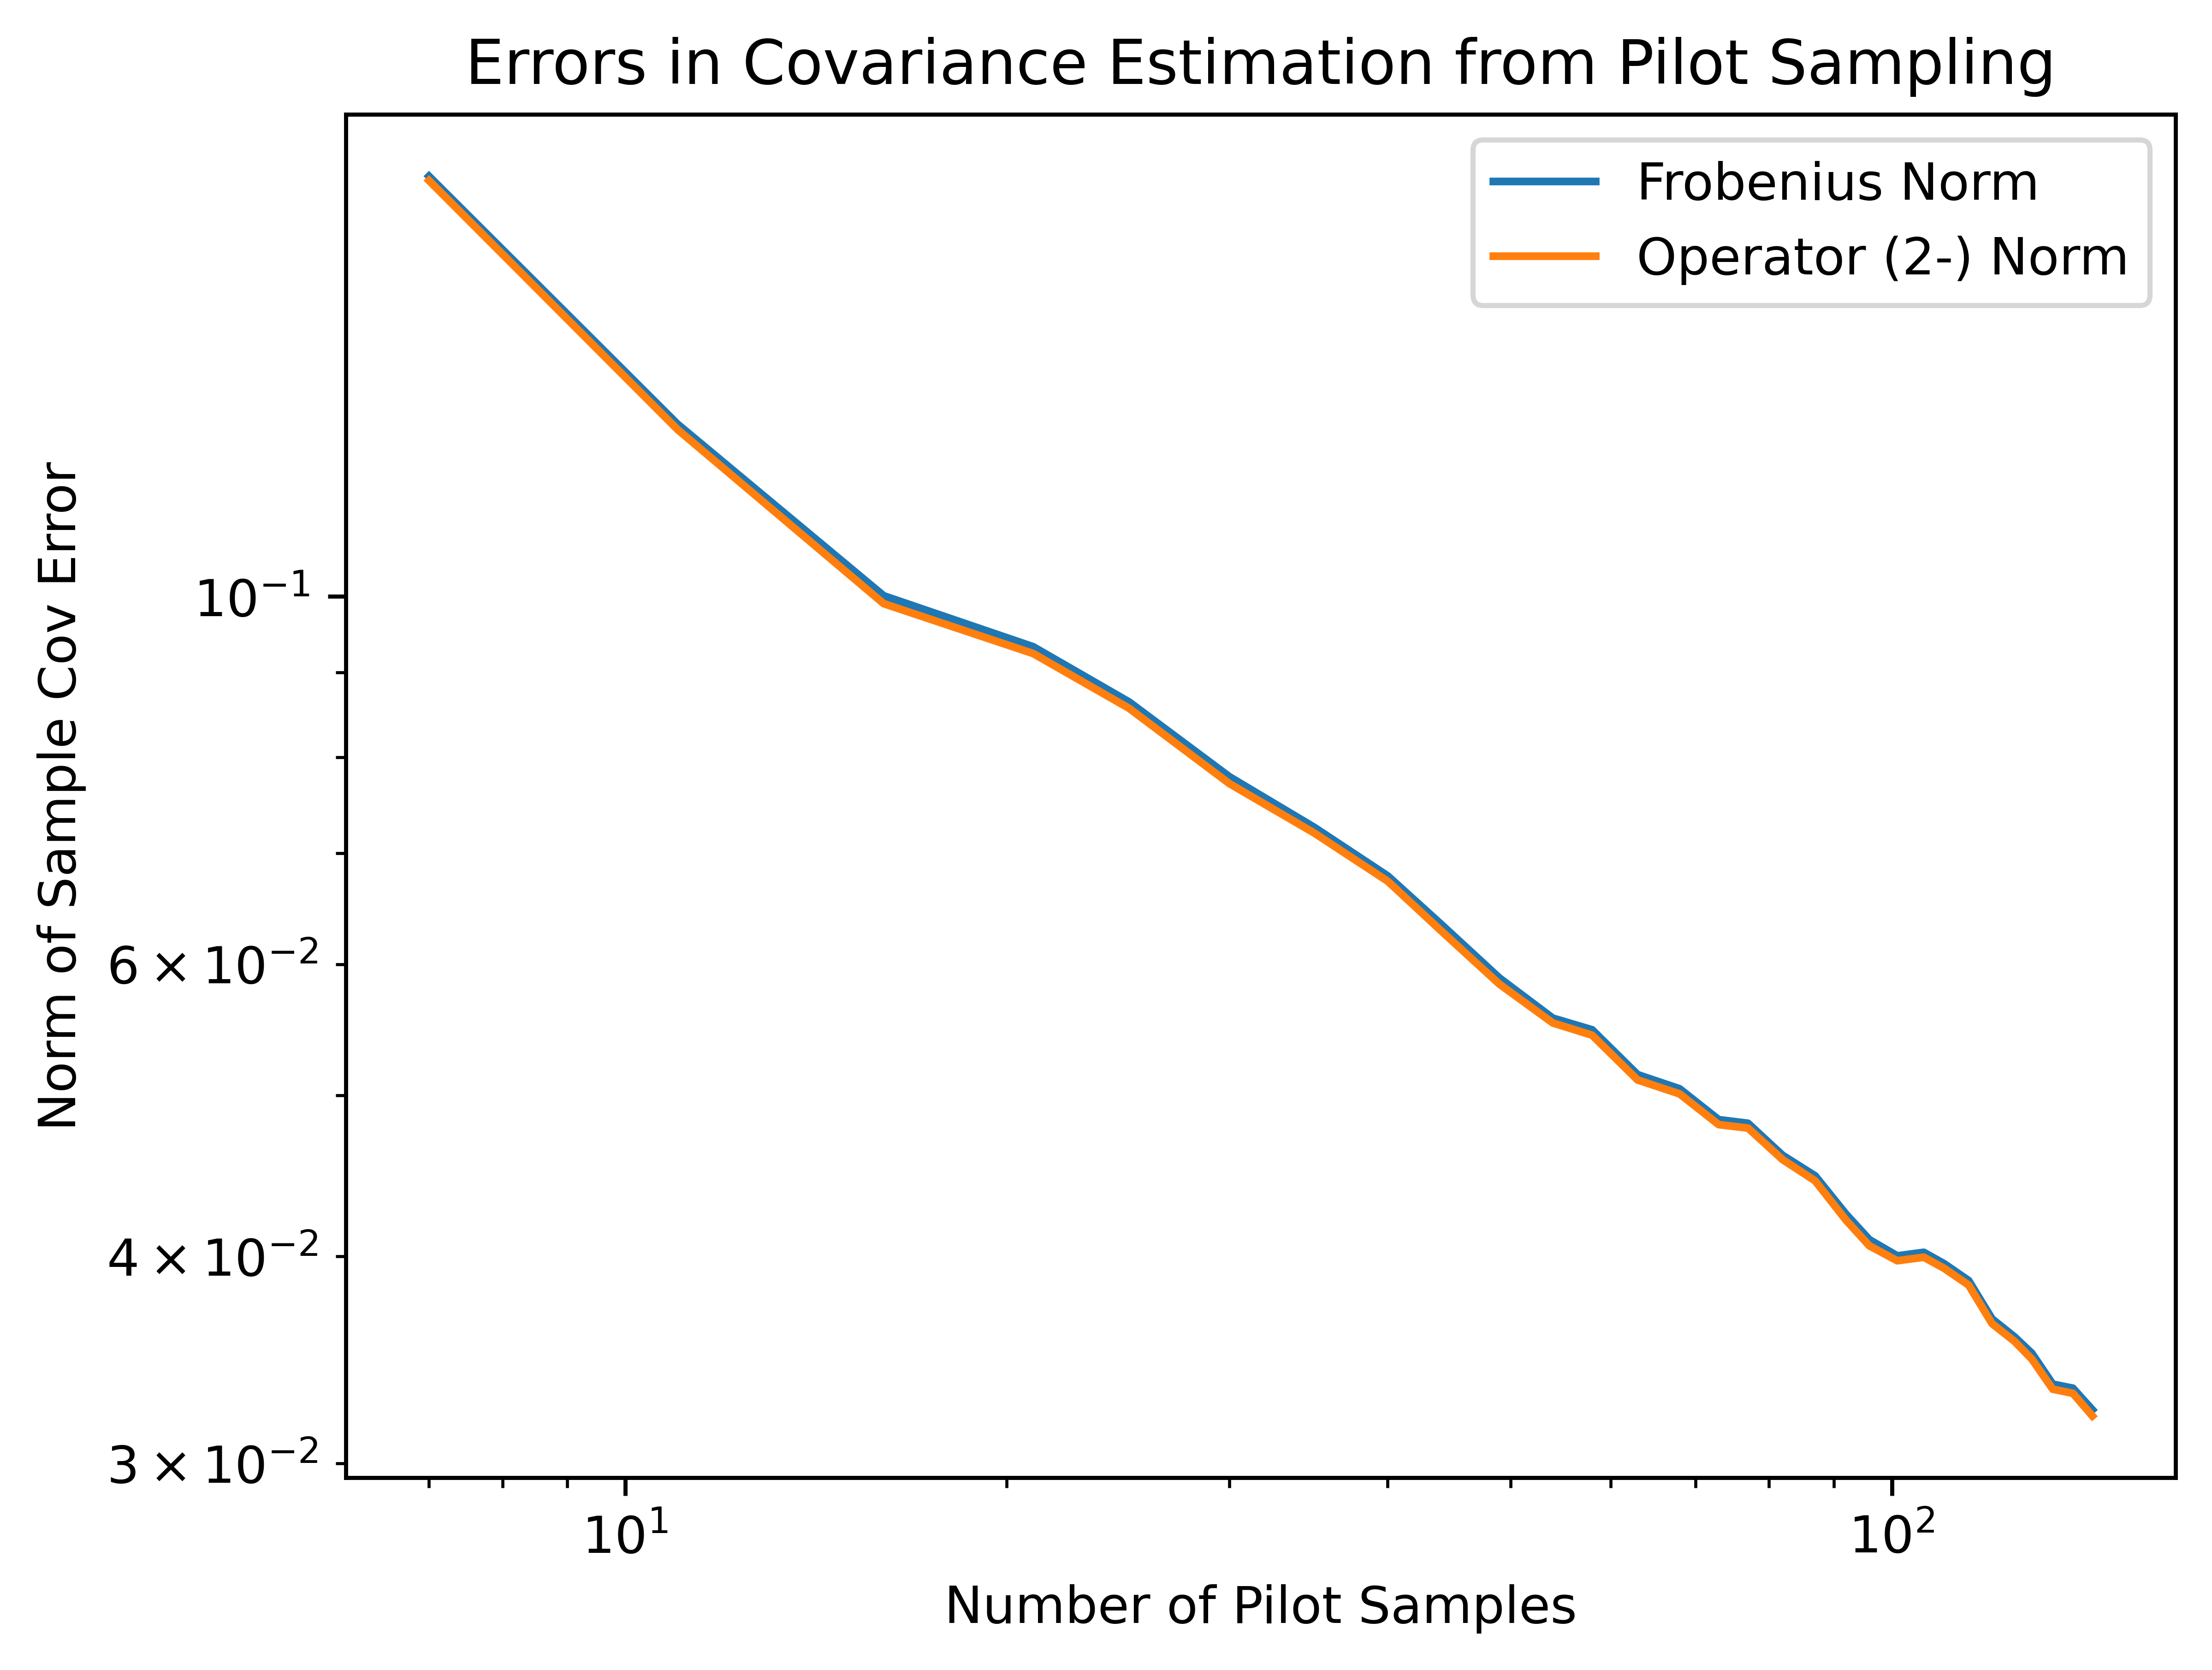
\includegraphics[width=0.45\textwidth]{fig/Cov_errs.png}
        \label{fig:cov_errs}
    \end{figure}
\end{frame}

\begin{frame}{Poor Covariance Estimates Hurt Estimation}
    The costs of poor covariance estimates are threefold:
    \begin{enumerate}
        \item Estimator variance is larger due to suboptimal sample allocation and weights,
        \item Projected variances from software tools will be inaccurate (false confidence in estimator results),
        \item Sample allocation optimization can often fail to converge under inaccurate covariance matrices.
    \end{enumerate}
\end{frame}

\begin{frame}{Poor Covariance Estimates Hurt Estimation}
    Budget is just 50 HF samples - accurate pilot sampling costs nearly the same as estimation.
    \begin{figure}
        \centering
        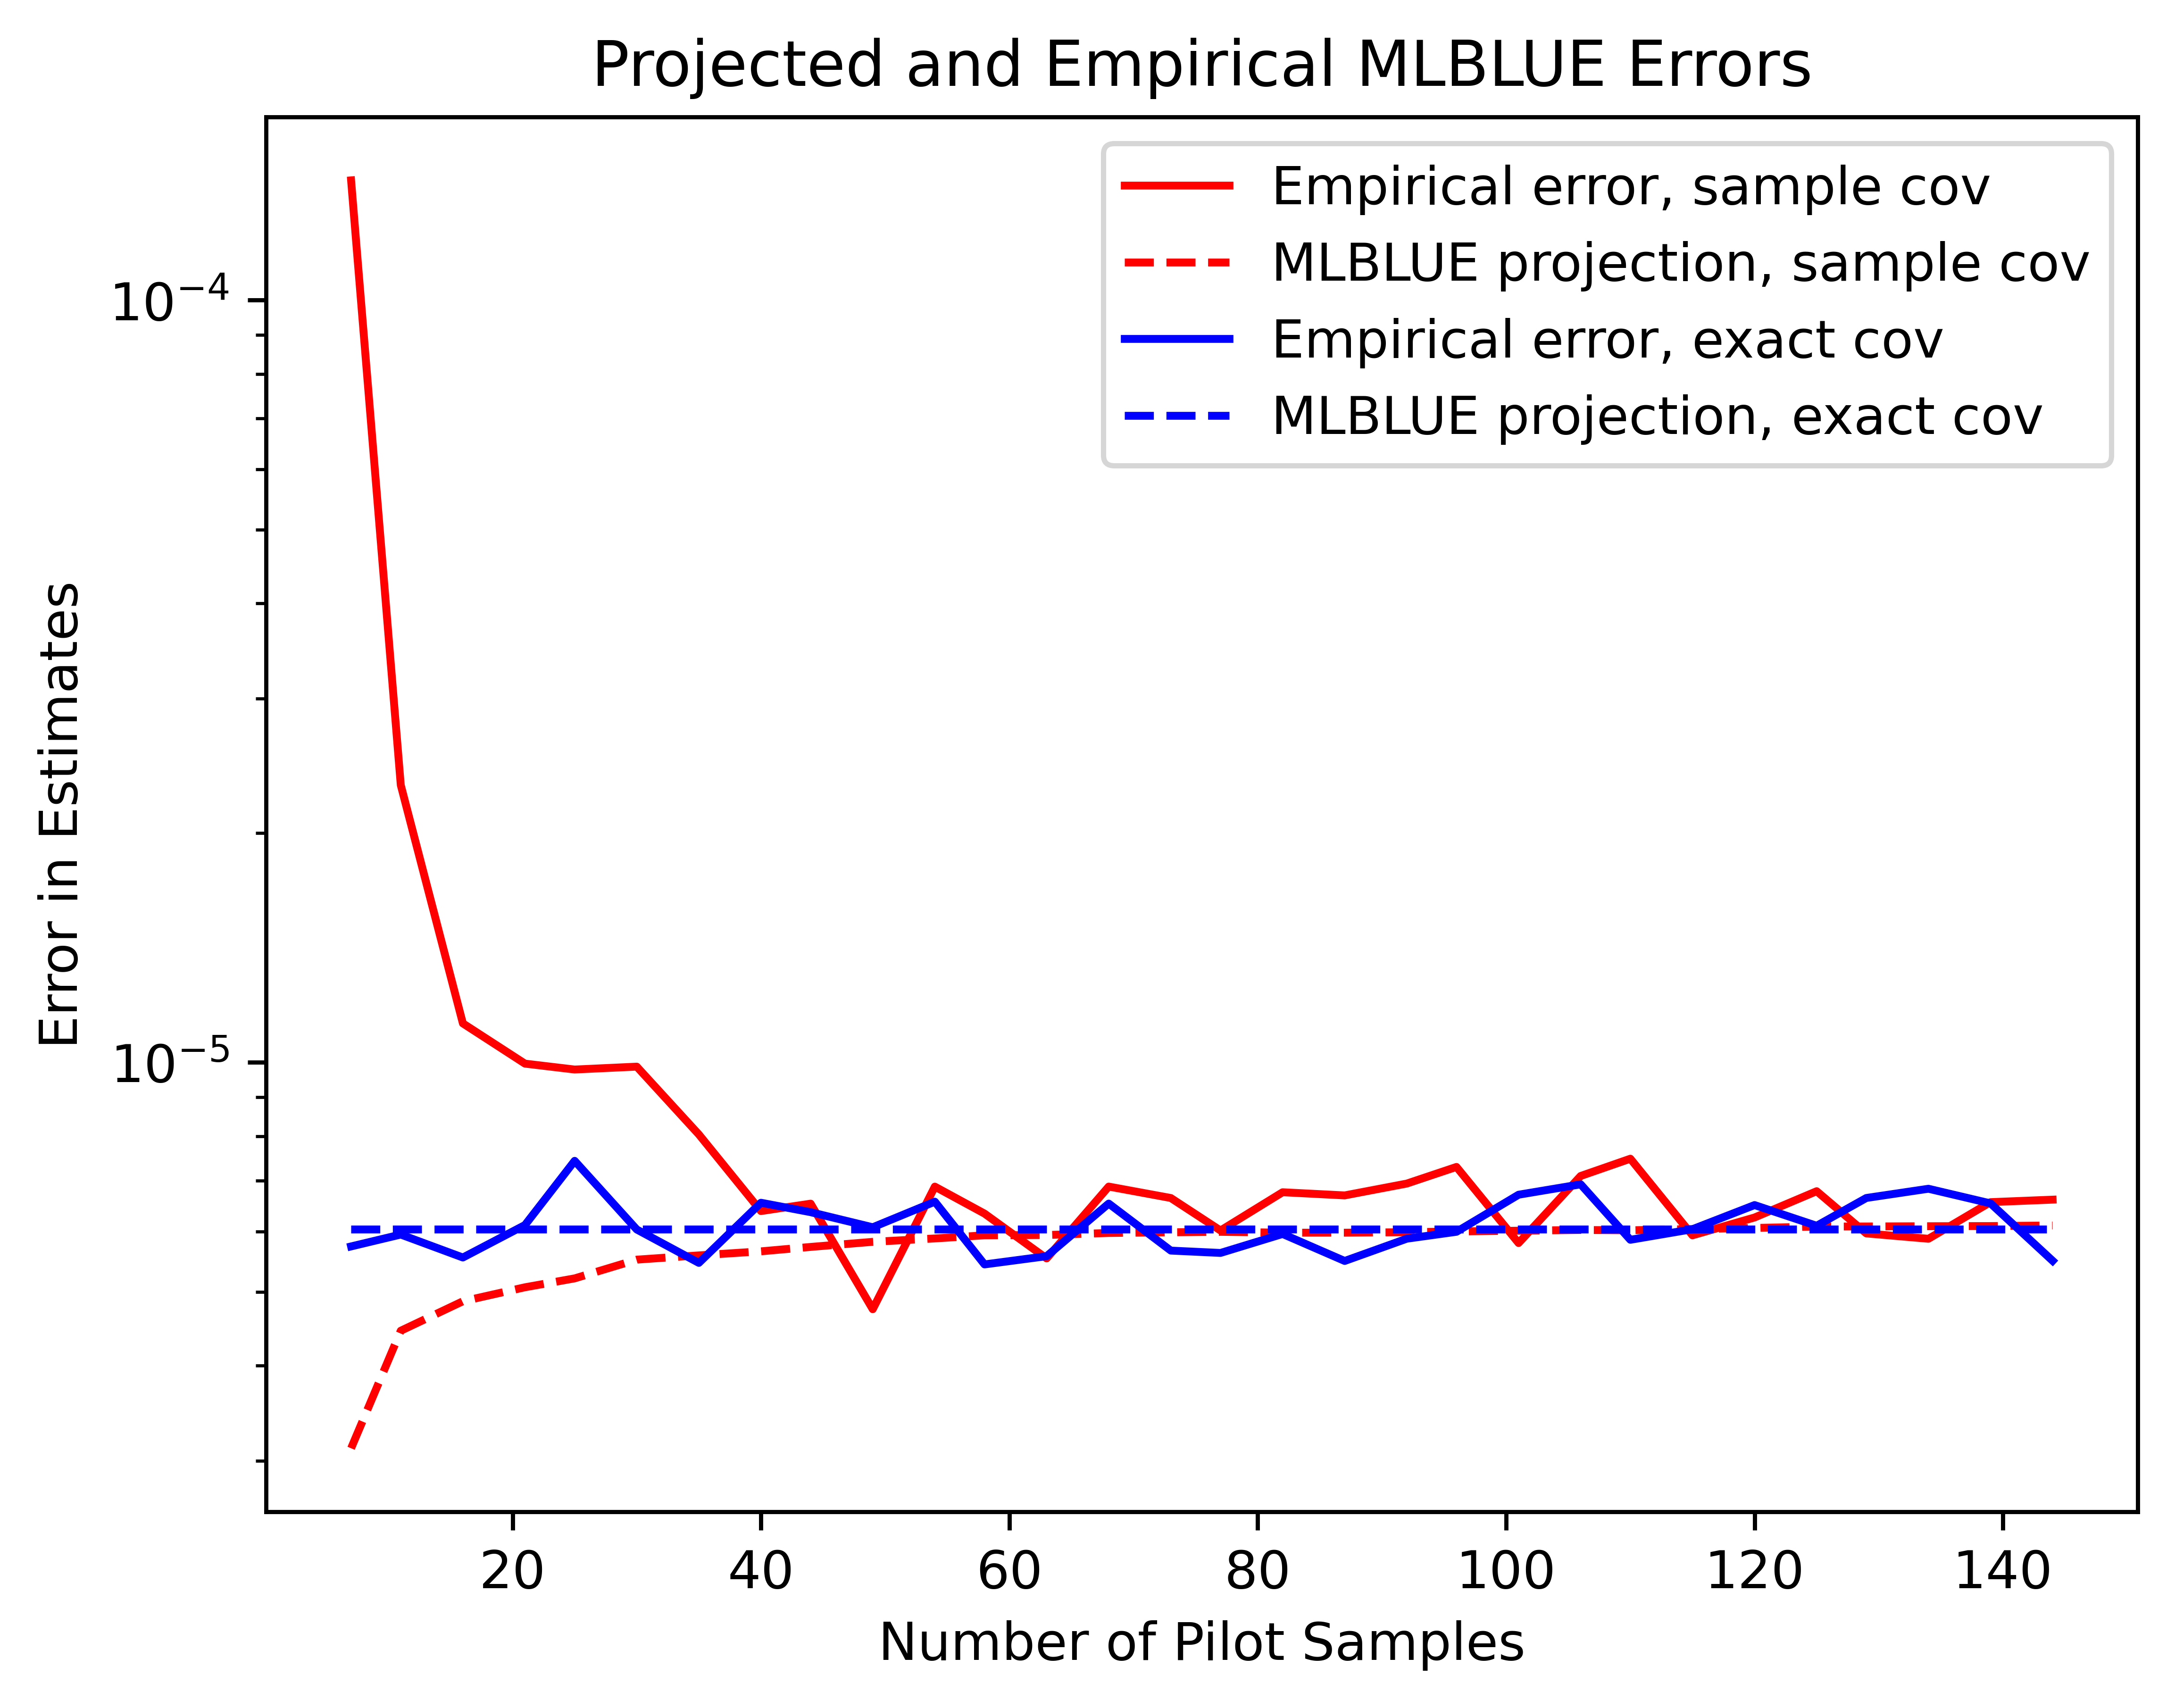
\includegraphics[width=0.7\textwidth]{fig/MLBLUE_errs.png}
        \label{fig:mlblue_errs}
    \end{figure}
\end{frame}

\begin{frame}{Poor Covariance Estimates Hurt Estimation}
    \begin{figure}
        \centering
        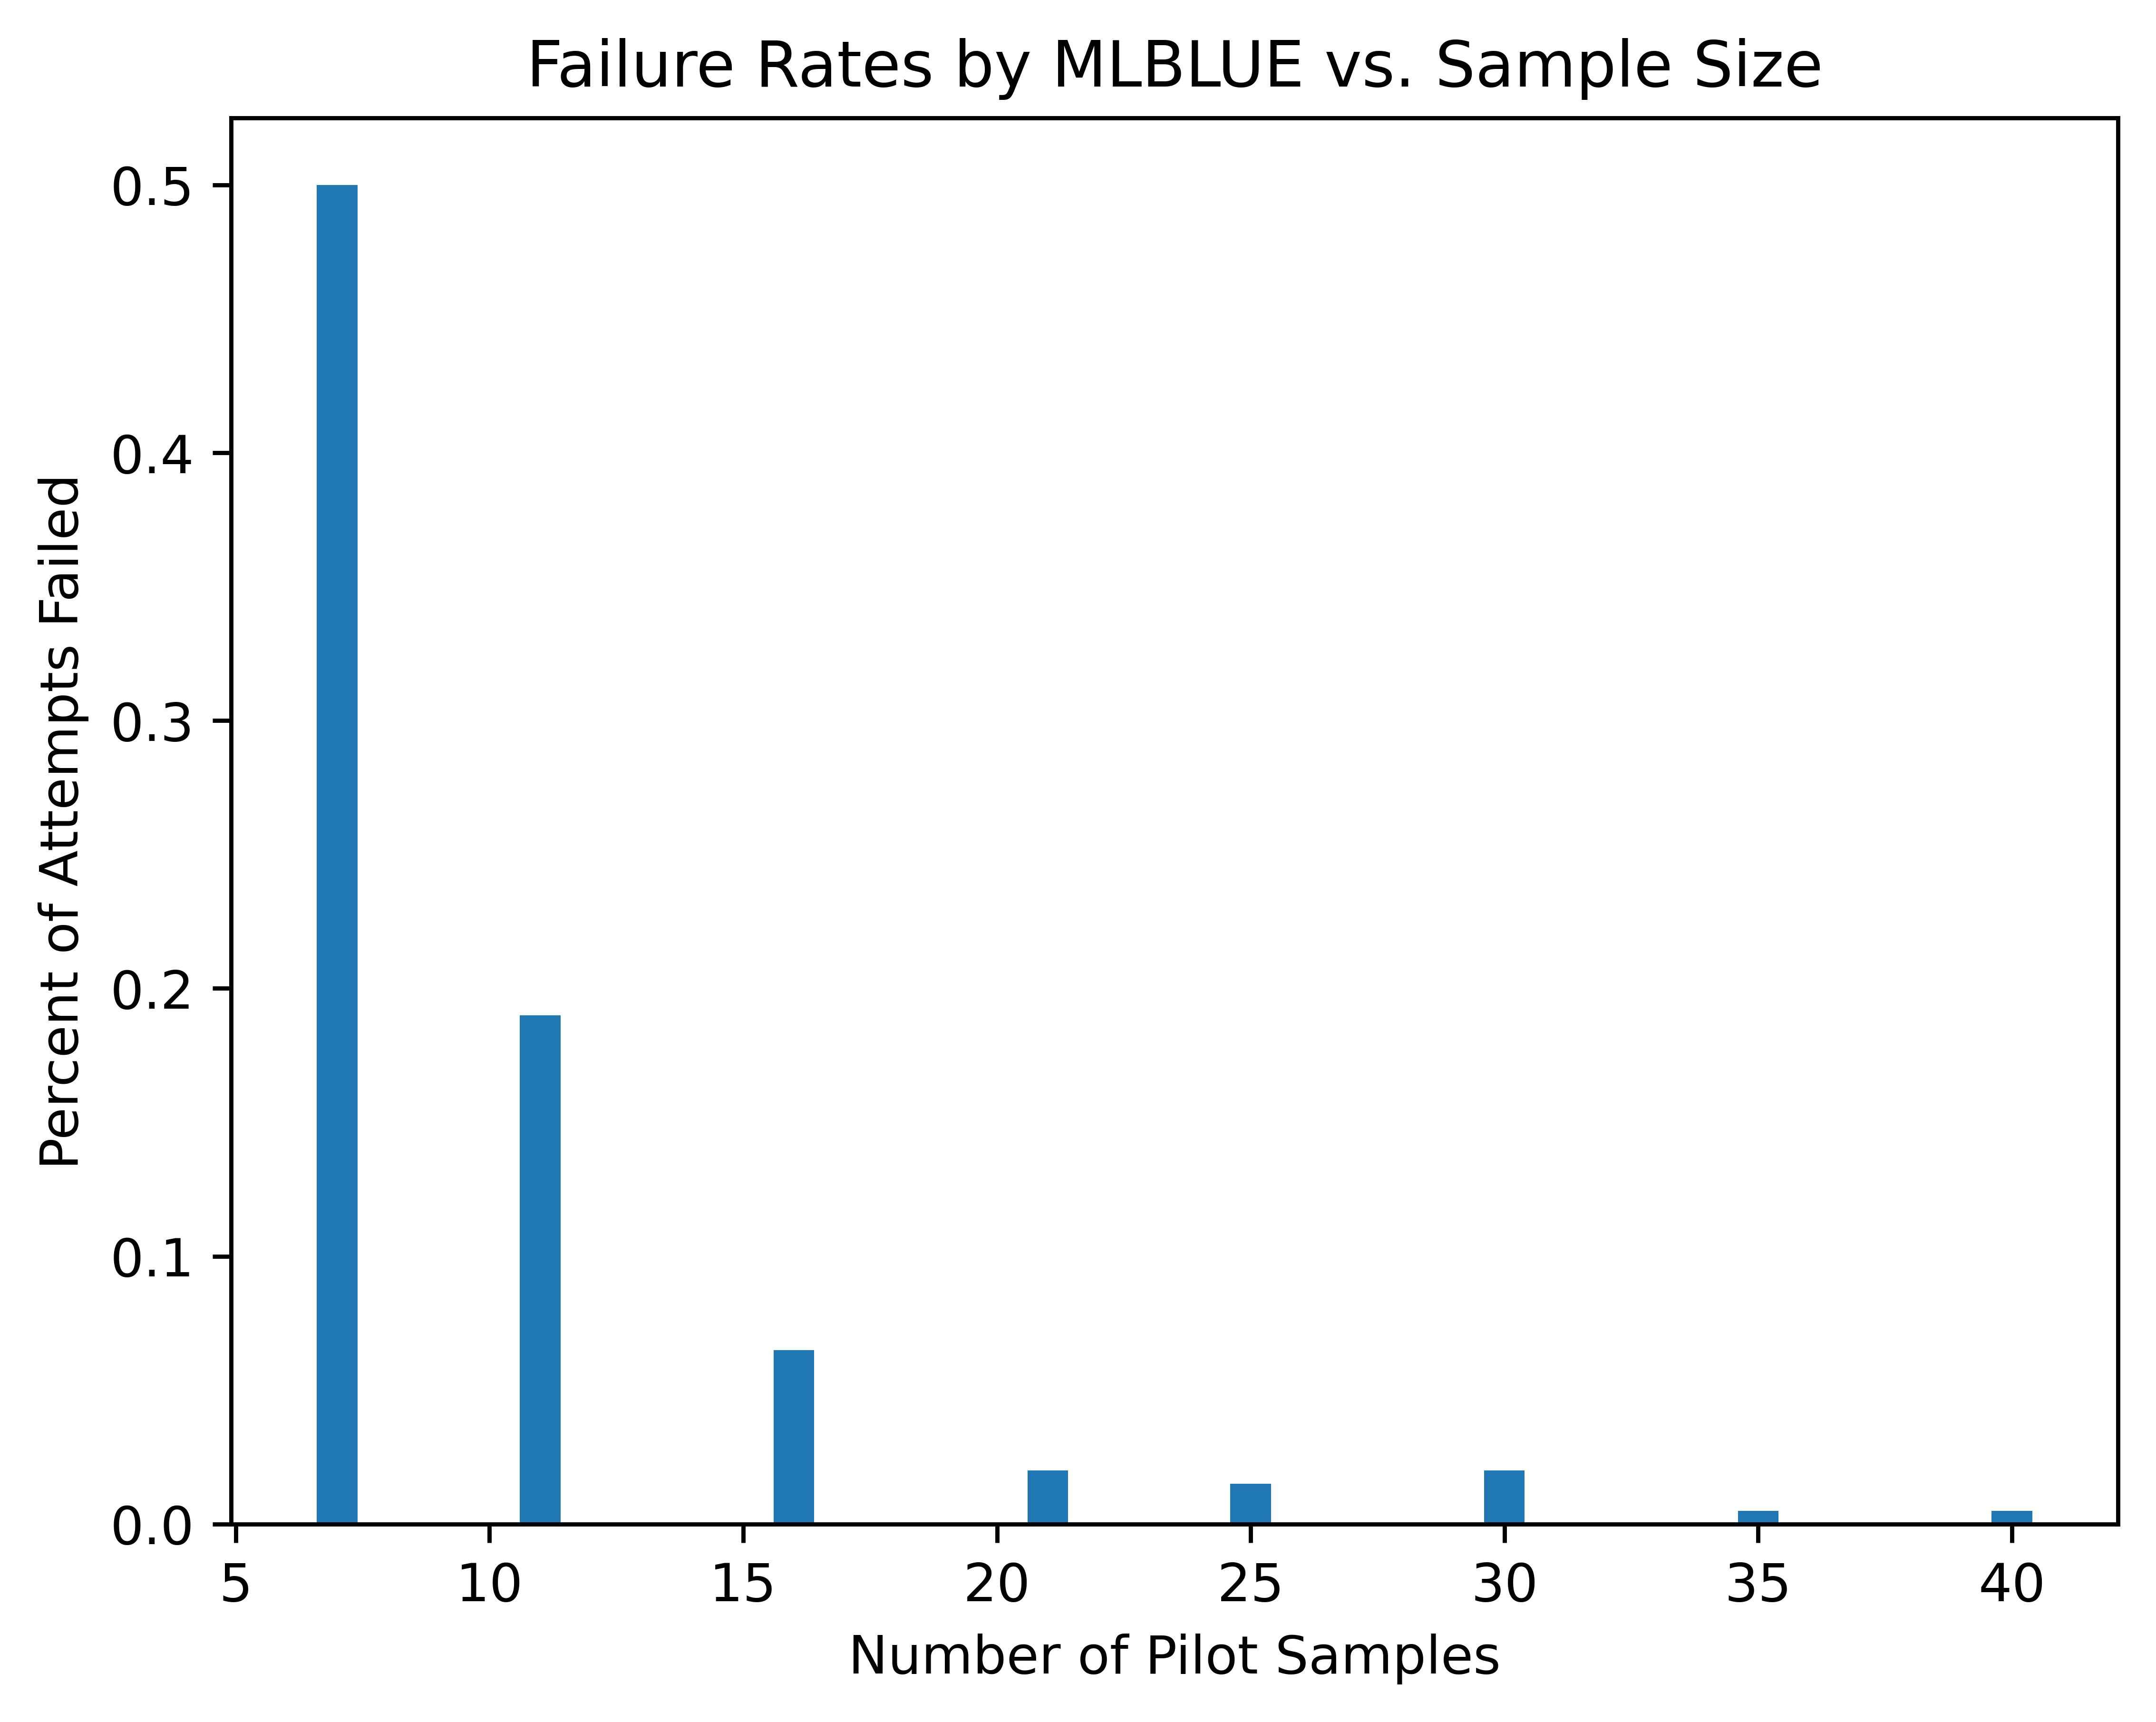
\includegraphics[width=0.8\textwidth]{fig/fail_rates.png}
        \label{fig:fail_rates}
    \end{figure}
\end{frame}

\section[Estimation]{Covariance Estimation in a Design Loop}
\begin{frame}{Covariance at Different Designs are Different}
    This is from the MFOED RANS turbulence closure model test case - I designed a one-size-fits-all estimator for use across the entire design space:
    \begin{enumerate}
        \item Take $nk$ pilot samples uniformly across the design space ($n$ samples at $k$ grid points),
        \item Compute $\hat{\Sigma}_{d}$ at each grid point $d_{1},...,d_{k}$,
        \item Average to get $\hat{\Sigma} = \mathbb{E}_{d}[\hat{\Sigma}_{d}] \approx \frac{1}{k}\sum_{i=1}^{k}\hat{\Sigma}_{d_{k}}$.
    \end{enumerate}
\end{frame}

\begin{frame}{Covariance Varies across Designs}
    The low-fidelity models are more poorly correlated in some regions of the design space:
    \begin{figure}
        \centering
        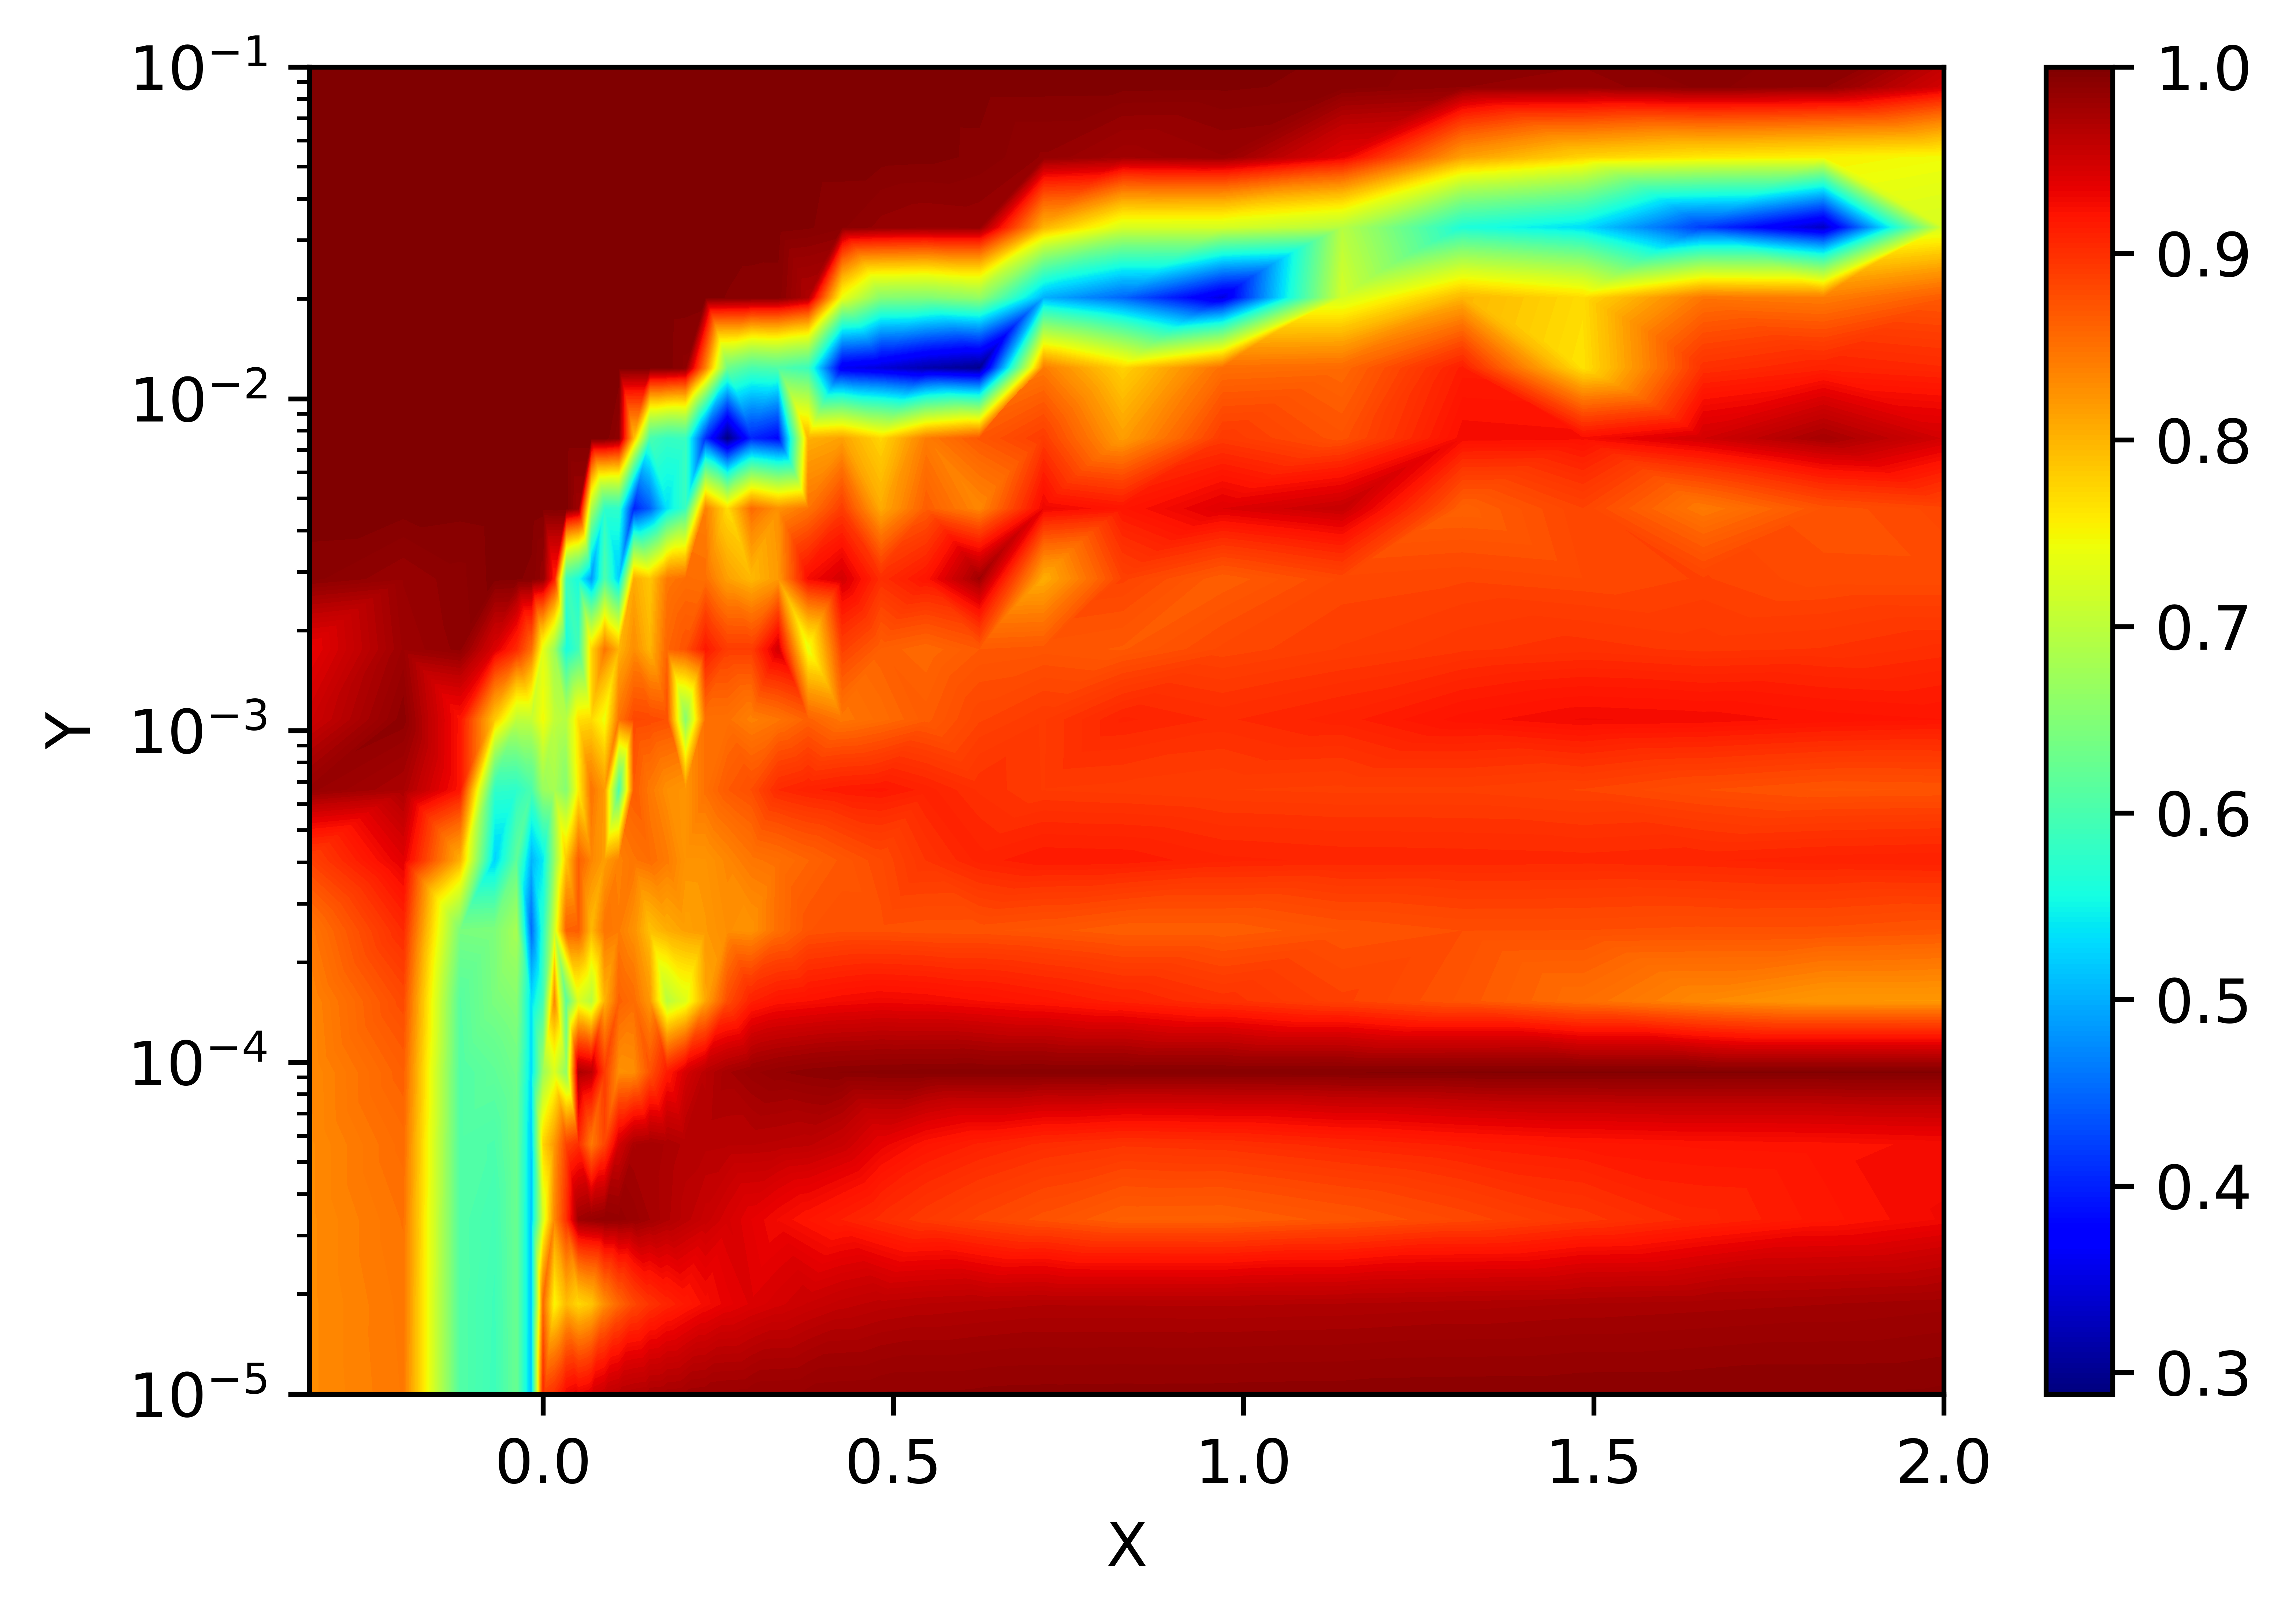
\includegraphics[width=0.7\textwidth]{fig/corrs_contour.png}
        \caption{Avg. LF Correlation to HF Model}
        \label{fig:corrs_contour}
    \end{figure}
\end{frame}

\begin{frame}{Estimator Variance Varies across Designs}
    As a result, our one-size-fits-all estimator projects the wrong estimator variance at some designs, and at the most important designs we ``get lucky" and see high estimator performance. What if our optimal design was at one of the poor performing regions in blue?
    \begin{figure}
        \centering
        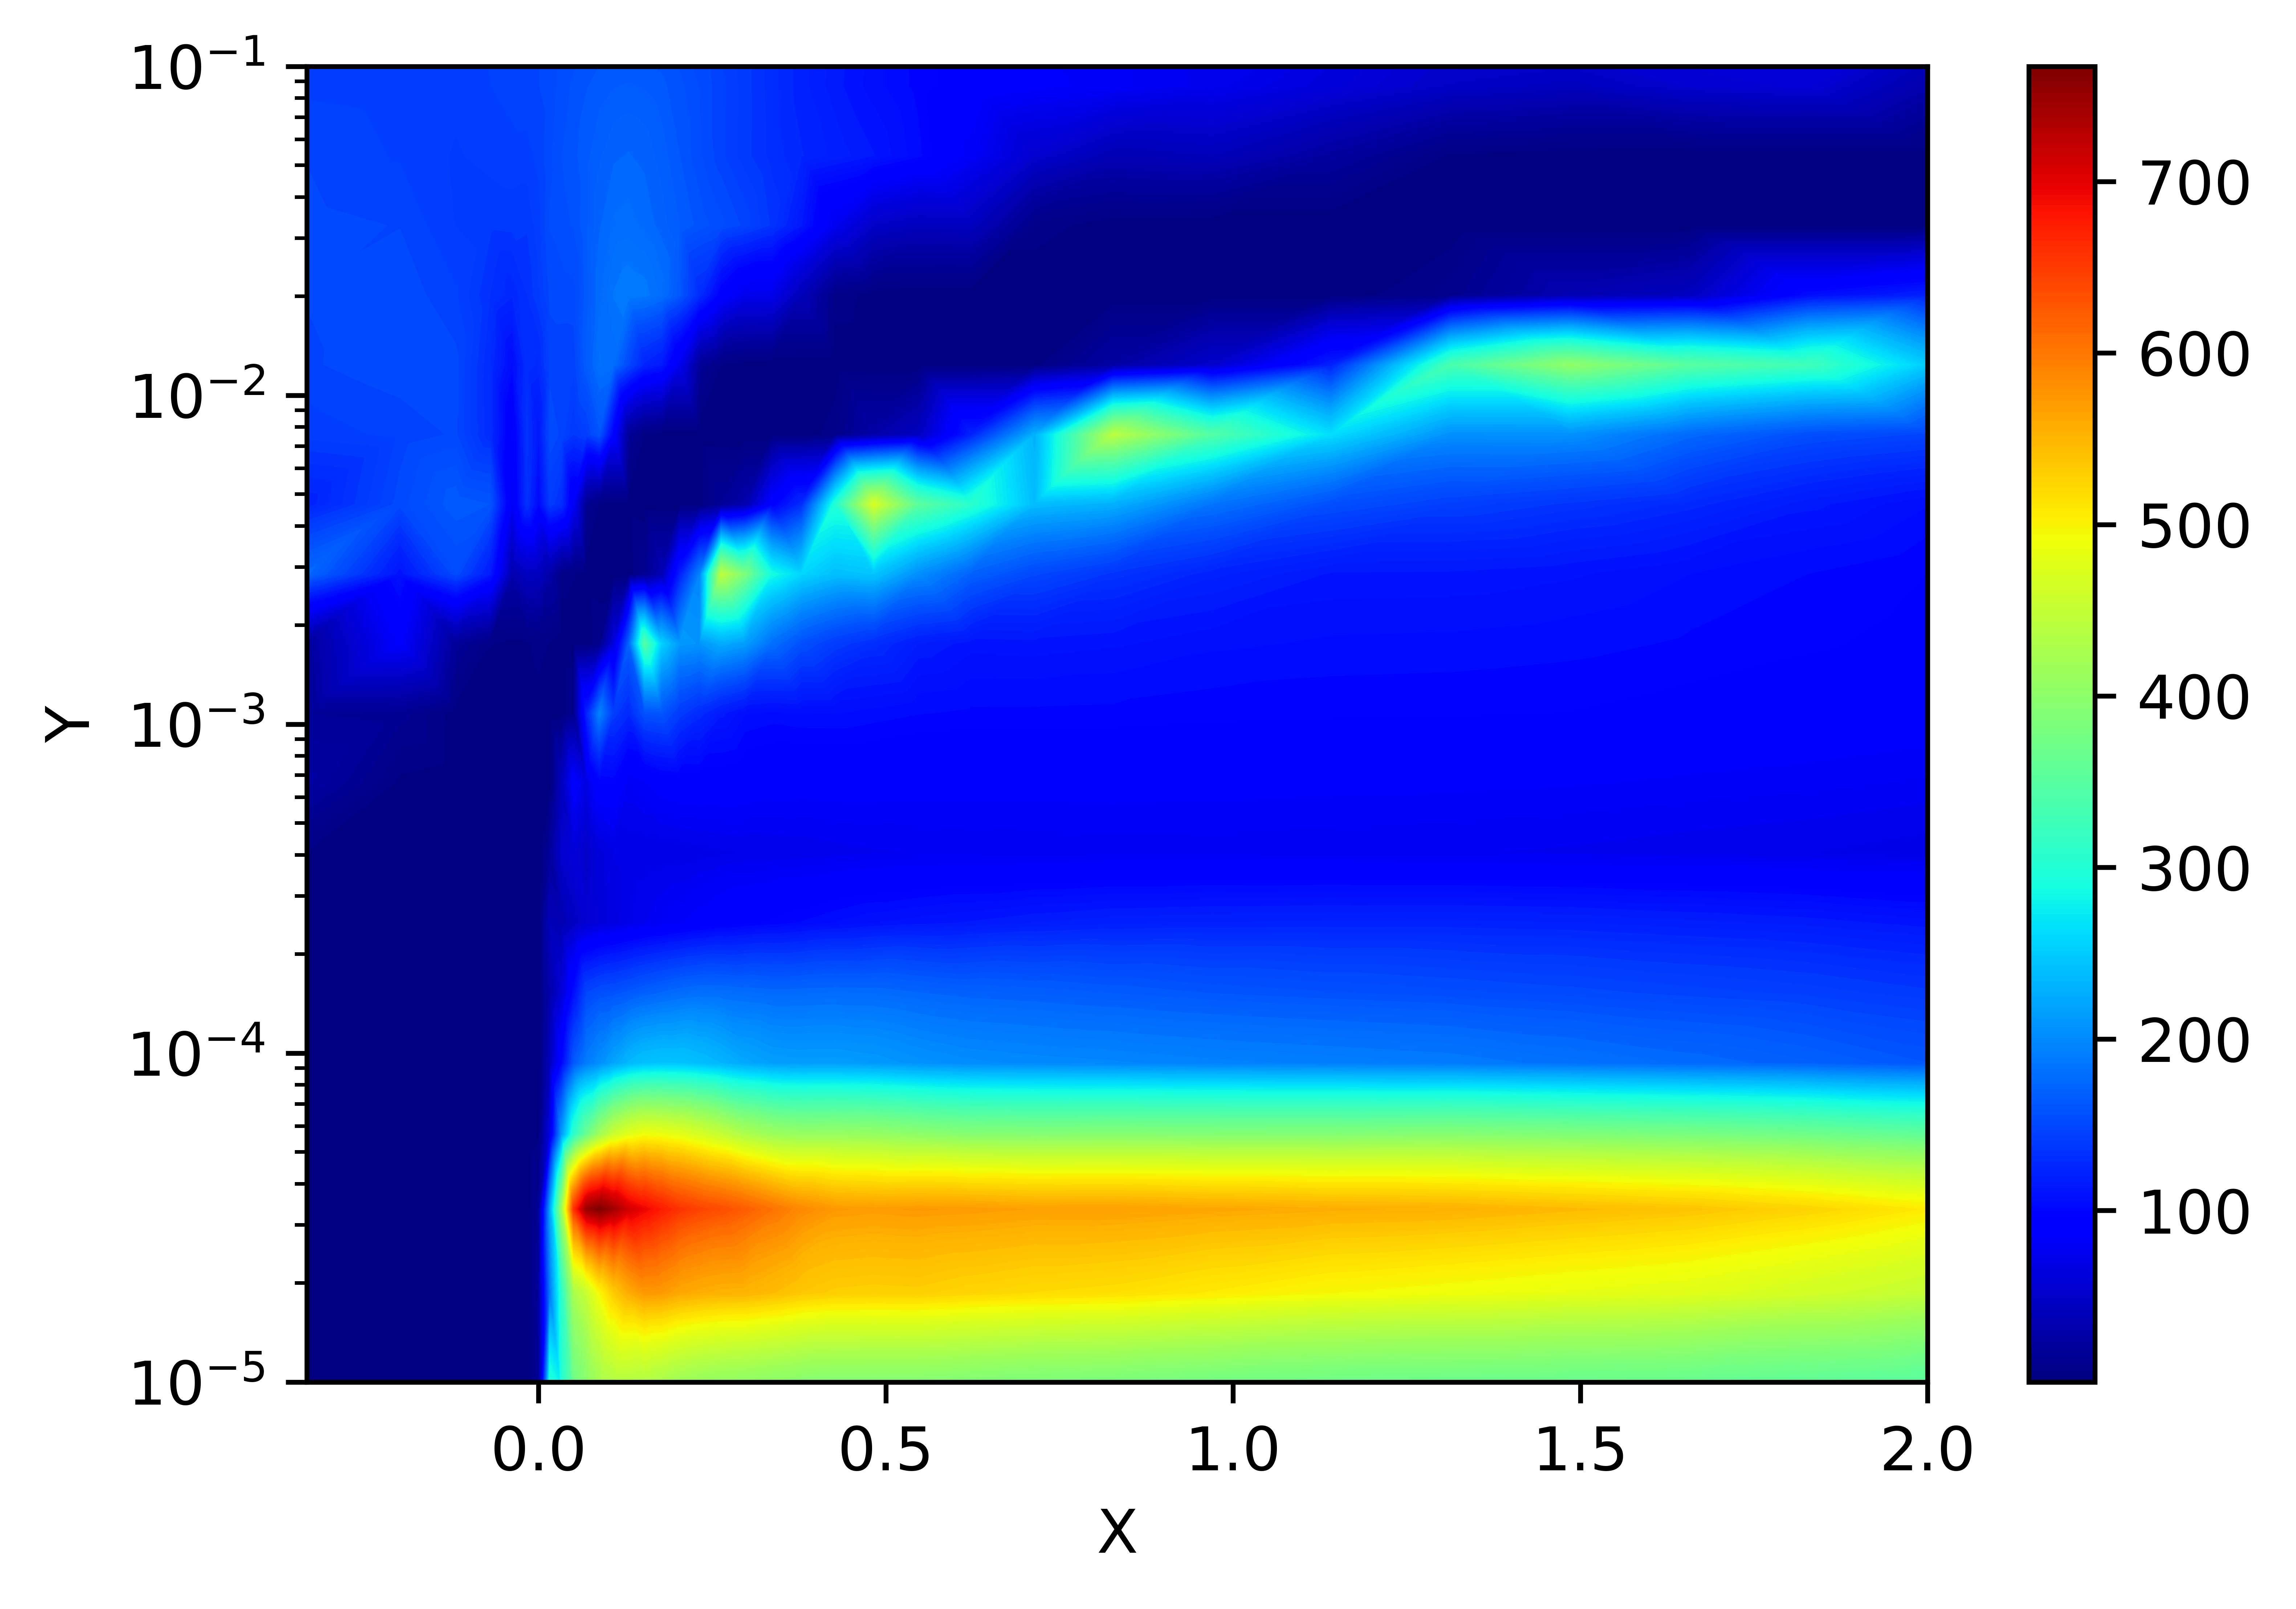
\includegraphics[width=0.5\textwidth]{fig/vrr_opt.png}
        \caption{Variance Reduction Ratios Across Domain}
        \label{fig:corrs_contour}
    \end{figure}
\end{frame}

\begin{frame}{A Possible Solution}
    During our pilot sampling (and estimator evaluations), can we use assumptions of smoothness to get covariance as a function of $d$?
    \begin{enumerate}
        \item Take some initial pilot samples across the domain,
        \item Estimate parameters of the covariance at each grid point, i.e. $\Sigma(\beta(d))$ where $\Sigma$ maps $\beta \in \mathbb{R}^{n_{\beta}} \rightarrow \mathbb{R}^{M\times M} \succeq 0$ and $\beta(d)$ maps $d \rightarrow \beta$,
        \item As optimization algorithm prompts near regions of the design space $d^{*}$, use $\Sigma(\beta(d^{*}))$ to design an optimal estimator, either taking more pilot samples or directly computing $\Sigma_{d^{*}}$.
    \end{enumerate}
\end{frame}

\section{Parametrization}
\begin{frame}{Existing Work - I}
    \cite{archakov2020}
    $\Sigma \in \mathbb{R}^{2 \times 2} \rightarrow v=(\log \sigma_1, \log \sigma_2, F(\rho))^T \in \mathbb{R}^3$
    
    $F(\rho) = \frac{1}{2}\log\left(\frac{1 + \rho}{1 - \rho}\right)$: Fisher transformation

    Required Properties For $n > 2$ Covariances:
    \begin{enumerate}
        \item Unique mapping
        
        \item Parametrization invariant to the ordering of variables.
    \end{enumerate}

    Solution: Matrix Logarithm for the correlation matrix $C$- $n(n-1)/2$ elements. $n$ variances are handled separately.

\end{frame}

\begin{frame}{Existing Work - II}
    Seek solution $x^{\ast}$ for symmetric $A$ s.t.
    $\log \operatorname{diag} \exp(A[x^{\ast}]) = 0 \in \mathbb{R}^n$

    by the convergence of the following iterative update from arbitrary $x_{0}$:

    $x_{k+1} = x_{k} - \log \operatorname{diag} \exp(A[x^{k}])$

    Example for $x_{0} \in \mathcal{U}(-2, 2)$:
    \begin{figure}
        \centering
        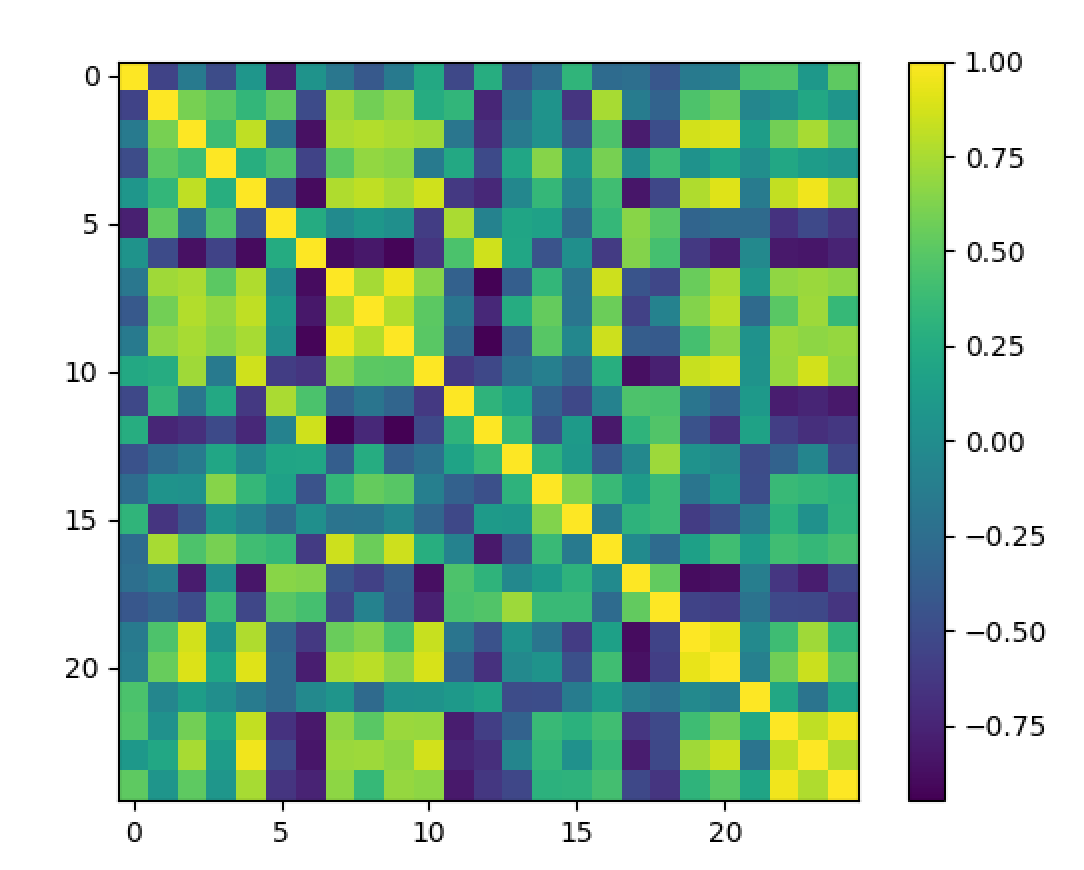
\includegraphics[width=0.45\textwidth]{fig/corr_log_transforms.png}
        \label{fig:corr_inversion}
    \end{figure}


\end{frame}

\begin{frame}{Non Parametric work}
\cite{Kidd2022}
Infer entries of covariance matrix directly from limited samples in spatial data.

Regularized inference on sparse Cholesky factors: \url{https://f-t-s.github.io/projects/cholesky/}
\begin{itemize}
    \item Construct sparsity sets $S_{\rho}$ around each point $x_i$ in domain i.e. neighbourhood such that $d(x_i, x_j) \leq \rho l_i$. $x_i$ chosen based on maximin ordering.
    
    \item Incomplete Cholesky factorization - ignore updates for entries outside of $S_{\rho}$
\end{itemize}

\textbf{Advantage}: Naive complexity $O(n^3)$ reduces to $O(n \log n \rho^d)$

\end{frame}

% \begin{frame}{Matching Parametric and Sample Estimates}


% \end{frame}

\section[Priors]{Prior Specification}
\begin{frame}{Existing Work - I}
    \begin{itemize}
    \item Inverse Wishart (IW) - conjugate prior:

    $f(\boldsymbol{\Psi}|m,\mathbf{V})=\frac{|\mathbf{V}|^{\frac{m}{2}}}{2^{\frac{mq}{2}}\Gamma_q(\frac{m}{2})}|\boldsymbol{\Psi}|^{-\frac{m+q+1}{2}}e^{-\frac{1}{2}\mathrm{tr}(\mathbf{V}\boldsymbol{\Psi}^{-1})}$
    
    
    In practice, performs poorly (over or under-estimate correlations) \cite{liu_comparison_2016}. Alleviated by a class of Shrinkage IW priors.

    \item SIW: \cite{berger_bayesian_2020}
    $p^{SIW}(\boldsymbol{\Sigma}|a,b,\mathbf{H})\propto\frac{etr(-\frac12\boldsymbol{\Sigma}^{-1}\mathbf{H})}{|\boldsymbol{\Sigma}|^a\prod_{i<j}(\lambda_j-\lambda_j)^b}$
    
    \item Separation Strategy with LKJ Priors:
    $\Sigma = S C S$ -  Impose prior on $C$, 1 scalar $\eta$ to tune correlation strength.

    \url{https://distribution-explorer.github.io/multivariate_continuous/lkj.html}

    \end{itemize}
\end{frame}


\begin{frame}{Modified LKJ Priors}
    \url{www.srmart.in/informative-priors-for-correlation-matrices-an-easy-approach}
    Correlation matrices with high correlations difficult to obtain from posterior estimates based on the LKJ Prior.

    $\implies$ Specify additional prior for off-diagonal elements of correlation:

    $$p(R) \propto \text{LKJ}(R | \eta = 1)\prod_{u}\mathcal{N}(R_u | \mu_u, \sigma_u)$$
\end{frame}


\begin{comment}

\section{Parametrization}
\begin{frame}{}
    
\end{frame}

\begin{frame}{Existing Work - II}


\end{frame}

\begin{frame}{Non Parametric work}


\end{frame}

\begin{frame}{Matching Parametric and Sample Estimates}


\end{frame}

\section{Specifying Informative Priors}
\begin{frame}{Existing Work - I}



\end{frame}

\begin{frame}{Existing Work - II}


\end{frame}


\begin{frame}{Modified LKJ Priors}
    Ref: 
    
\end{frame}


% \section{Inference and Active Learning}




% \section{Toy examples}



% \section{Application}
% \begin{frame}{Backup: Bonus}
\end{comment}

\begin{frame}[allowframebreaks]
    \frametitle{References}
    \bibliographystyle{chicago}

    %\bibliographystyle{IEEEtran}
    \bibliography{feb_13}
\end{frame}

\section{Backup}
\begin{frame}{}
\begin{center}
    \Large{Thank you!}
\end{center}
        
\end{frame}

% Nice 15 minute read on the subject and the philosophy: \url{https://www.stochasticlifestyle.com/how-to-train-interpretable-neural-networks-that-accurately-extrapolate-from-small-data/}

% \end{frame}
% \begin{frame}{Backup 5: Implementation}
% Some other day.
% \end{frame}
\end{document}
